\documentclass[a4paper]{report} %Always requireed
%========================================================================
% preamble to declare kackges used in the document
%========================================================================
%Packages that will be used

%To use a block comment in a document
\usepackage{comment} 
\begin{comment}
	Test a block comment 
\end{comment}
\usepackage{enumitem}
\usepackage{amssymb}
\usepackage{graphicx}
\graphicspath{{Figures/}}

\usepackage{ragged2e}
%------------------------------------------------------------------------
\usepackage{fontspec}
%Either Xelatex or Lualatex is required as a default complier
%To learn more about "fontspec" package: https://ctan.org/pkg/fontspec?lang=en 
%========================================================================
%To declare a document title and an author(s) 
\title{This is a title of my first document}
\author{Firstname Lastname}

\begin{comment}
	\author{
		LastName1, FirstName1\\
		\texttt{first1.last1@xxxxx.com} 
		\and
		LastName2, FirstName2\\
		\texttt{first2.last2@xxxxx.com}
		\and
		LastName3, FirstName3\\
		\texttt{first3.last3@xxxxx.com}
		\and
		LastName4, FirstName4\\
		\texttt{first4.last4@xxxxx.com}
	}
\end{comment}

%document
\begin{document}
	\maketitle
	%Put your text in a body of your document here... 
	\setcounter{chapter}{1}
	\chapter*{Chapter 1}
	
	\section{Introduction}
	
	\section{Objectives}
	\begin{itemize}
		\item OBJ 1
		\item OBJ 2
		\item OBJ 3
		\begin{itemize}
			\item [-] OBJ 3-1
			\item [-] OBJ 3-2
			\item [-] OBJ 3-3
		\end{itemize}
	
	\end{itemize}

	\section{Scopes}
	\begin{itemize}
		\item [$\blacksquare$] SCP 1
		\item [$\blacksquare$] SCP 2
		\item [$\blacksquare$] SCP 3
	\end{itemize}
	
	\section{Expected Results}
	\begin{enumerate} [label=\arabic*)]
		\item Expected Result 1
		\begin{enumerate} [label=\textit{\roman*)}]
			\item \textit{Expected Result 1.1}
			\item \textit{Expected Result 1.2}
			\item \textit{Expected Result 1.3}
		\end{enumerate}
		\item Expected Result 2
		\item Expected Result 3
	\end{enumerate}
	\section{Timeline}
	\begin{figure}[!h]
		\noindent\Centering
		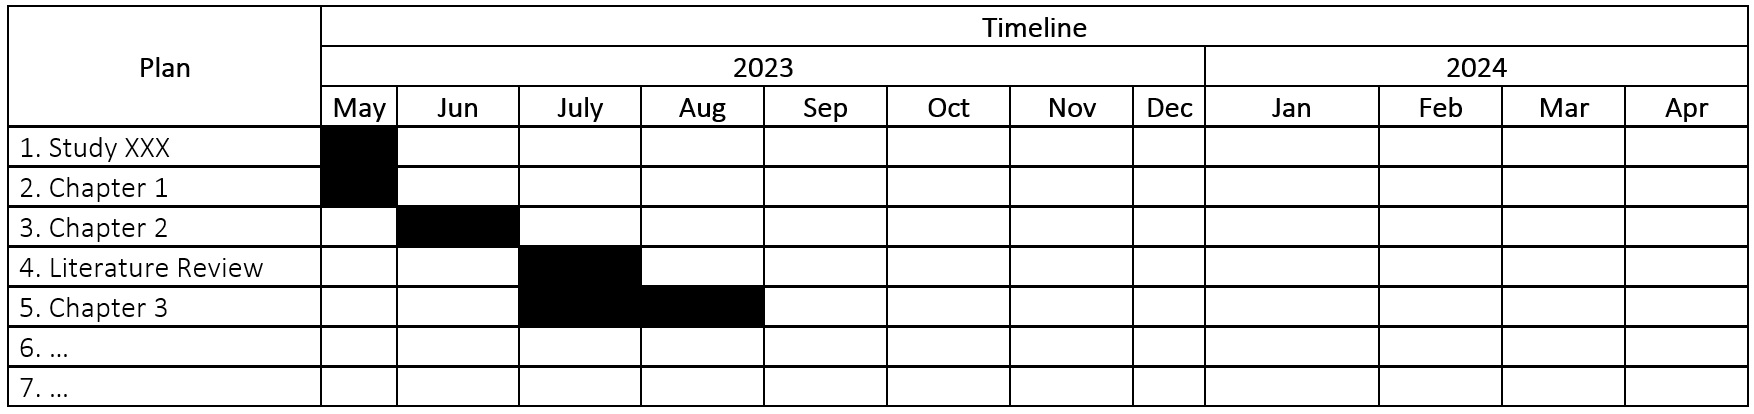
\includegraphics[width=1\textwidth]{Timeline}
		\caption{Mahidol University.}
		\label{fig:MU Logo}
	\end{figure}
\end{document}
%========================================================================